\documentclass[12pt]{article}
\usepackage{graphicx}
\usepackage{setspace}
\usepackage{geometry}
\usepackage{changepage}
\usepackage{float}

% Convert references, table of contents and list of figures to links.
\usepackage[colorlinks=false,pdfborder={0 0 0}]{hyperref}

% Make captions look better.
\usepackage[labelfont={bf, it},textfont=it]{caption}

% Support for references.
\usepackage[backend=biber,style=ieee]{biblatex}
\addbibresource{refs.bib}

% Page settings
\geometry{margin=1in}

% Document metadata
\title{CNG 495 Term Project Proposal}
\date{October 19, 2025}

% 1.5 line spacing entire document
\onehalfspacing 



\begin{document}

% === Title page ===
\begin{titlepage}
    \begin{center}
        \Huge\bfseries CNG 495 Cloud Computing \\ Fall 2025-2026 Semester \\ Term Project Proposal
    \end{center}

    \vfill
    \vfill
    
    {
        \large
        \begin{tabular}{@{} l l @{}}
            \textbf{Project Name}: & RFID-based Attendance System \\
            \textbf{Team Members}: & Can Özkan  - 2638112 \\
                                   & Umut Şen - 2585420 \\
        \end{tabular}
    }

    \vfill
\end{titlepage}


\renewcommand{\contentsname}{Table of Contents} % Rename "Contents" to "Table of Contents"
\tableofcontents
\listoffigures
\newpage



\section{Project Description}
Our project aims to simplify and automate the process of taking attendance using student ID cards by reducing human interaction. Our system consists of an NFC reader hardware, a cloud server that processes attendance \& timetable data, and two distinct web-based user interfaces, for instructors and administrators.\par

Instructors can login to the system using their METU credentials. The interface lets them see how many registered students have arrived, how many are absent and the total number of students registered to the classroom, in a simple interface. In case of a hardware failure, or simply a student forgetting to scan their ID, the instructor can mark a student present too, during or after the lecture hours. Similarly, the instructor can mark a student absent even if the ID card was scanned.\par

The administration panel is strictly to be used by administrators (such as the registrar's office) to monitor the RFID readers, assign them to classrooms and view system logs.\par



\section{Implementation}
Times of each lecture, and in which classroom they are taking place are automatically pulled from the university’s timetable system. When a student arrives at the classroom, they are required to scan their ID cards to the RFID reader. Scanned RFID data is then sent to the cloud server to register attendance. RFID reader has both visual and audio elements to give feedback. Students must scan their ID until the lecture time is over for their attendance to be valid. This process can be seen on \autoref{fig:activity}.\par

Our project will use ASP.NET as the backend framework, Supabase as the database and React on GitHub Pages for the frontend design of the cloud part. For the hardware part, we utilize an RC522 RFID module to scan ID cards, ESP32-DevKit-V1 module to transmit ID to the cloud, an LCD screen and a buzzer to provide feedback.\par

Interaction between services of our project can be seen on \autoref{fig:context}.

\begin{figure}[H]
    \centering
    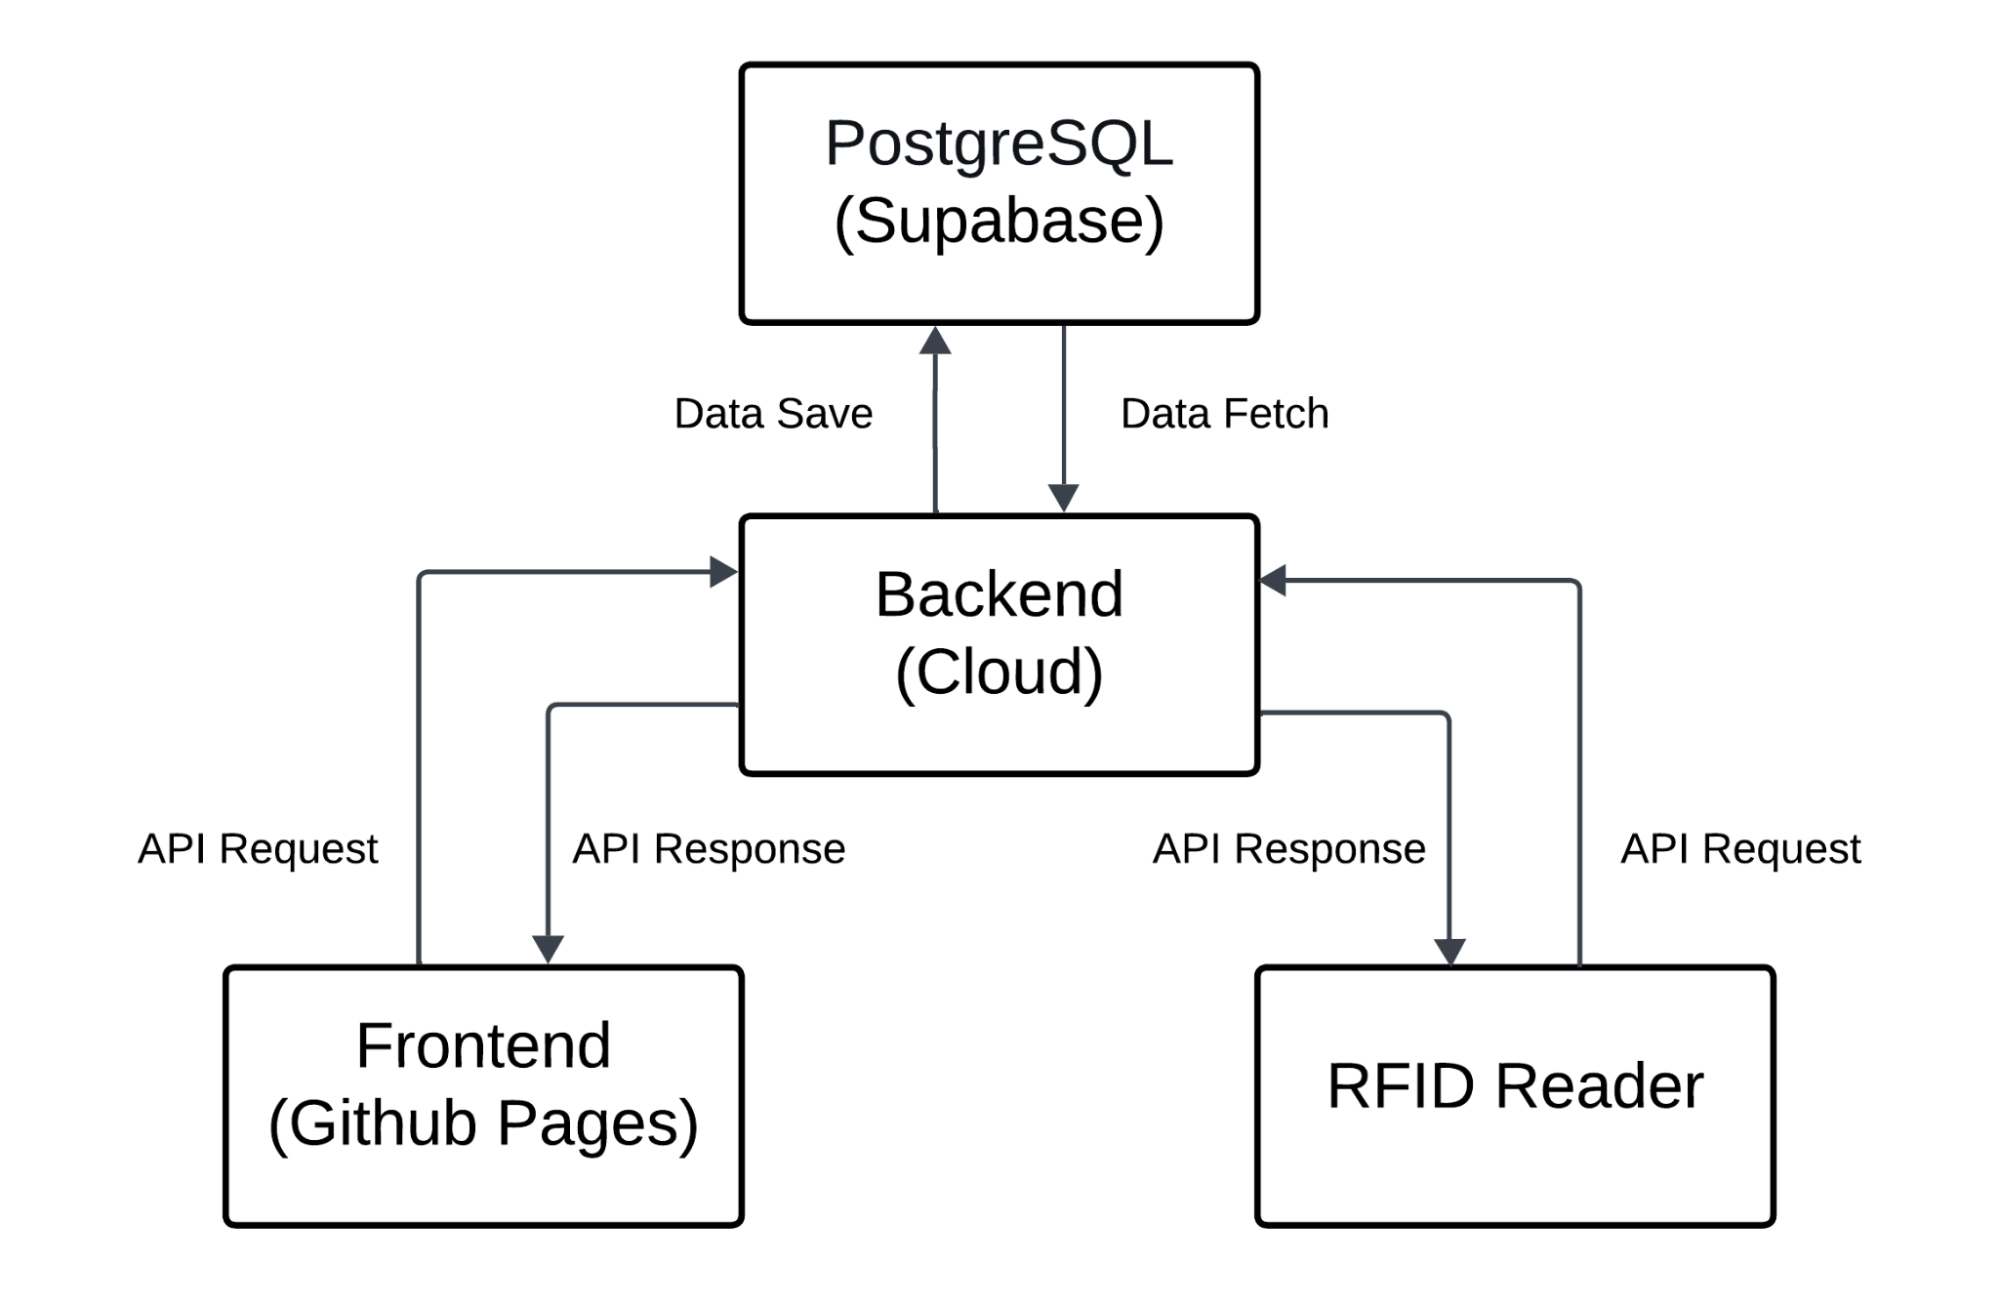
\includegraphics[width=\linewidth]{context.png}
    \caption{System interactions.}
    \label{fig:context}
\end{figure}



\section{Delivery Models}

\subsection{Platform-as-a-Service (PaaS)}
Frontend for our project will be hosted on GitHub Pages, and the database will be hosted on Supabase.\supercite{github-pages,supabase-docs}

\subsection{Infrastructure-as-a-Service (IaaS)}
Our backend will run on a virtual private server with a Linux-based operating system.\supercite{vps-com-tr}



\newpage
\section{Data Types}
Our project utilizes various data types to exchange and store information. Data types used in our project are detailed below, categorized by the group they’re used in.

\begin{itemize}
    \item \textbf{Text:} Student full name, Instructor full name, Classroom name, Hardware IP address
    \item \textbf{Number:} Student ID number
    \item \textbf{Timestamp:} Lecture start/end timestamps
    \item \textbf{Binary:} ID card data, hardware keys
\end{itemize}



\section{Computation}
Following computations are made throughout the lifetime of our system:

\begin{itemize}
    \item \textbf{Attendance Recording:} Student attendance is recorded and present \& absent student counts are calculated.
    \item \textbf{User Authentication:} Credentials of parties accessing our system are verified through the METU system.
    \item \textbf{Hardware Authentication:} To prevent unauthorized attendance recording to our system, we check the authenticity of requests coming from all RFID readers.
\end{itemize}



\section{Expected Contribution}
\begin{itemize}
    \item \textbf{Hardware Design \& Implementation:} Can Özkan
    \item \textbf{Database Design:} Both students
    \item \textbf{Backend Development:} Both students
    \item \textbf{Frontend Development:} Umut Şen
\end{itemize}



\newpage
\section{Diagrams}
This section contains various diagrams that visualize how our system works.

\subsection{Activity Diagram}

\begin{figure}[H]
    \centering
    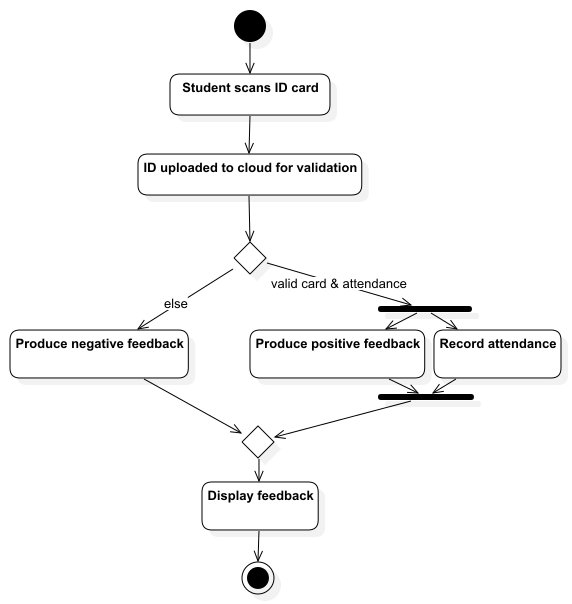
\includegraphics[width=\linewidth]{activity.png}
    \caption{Student ID \& attendance verification process.}
    \label{fig:activity}
\end{figure}


\newpage
\subsection{Use Case Diagram}

\begin{figure}[H]
    \centering
    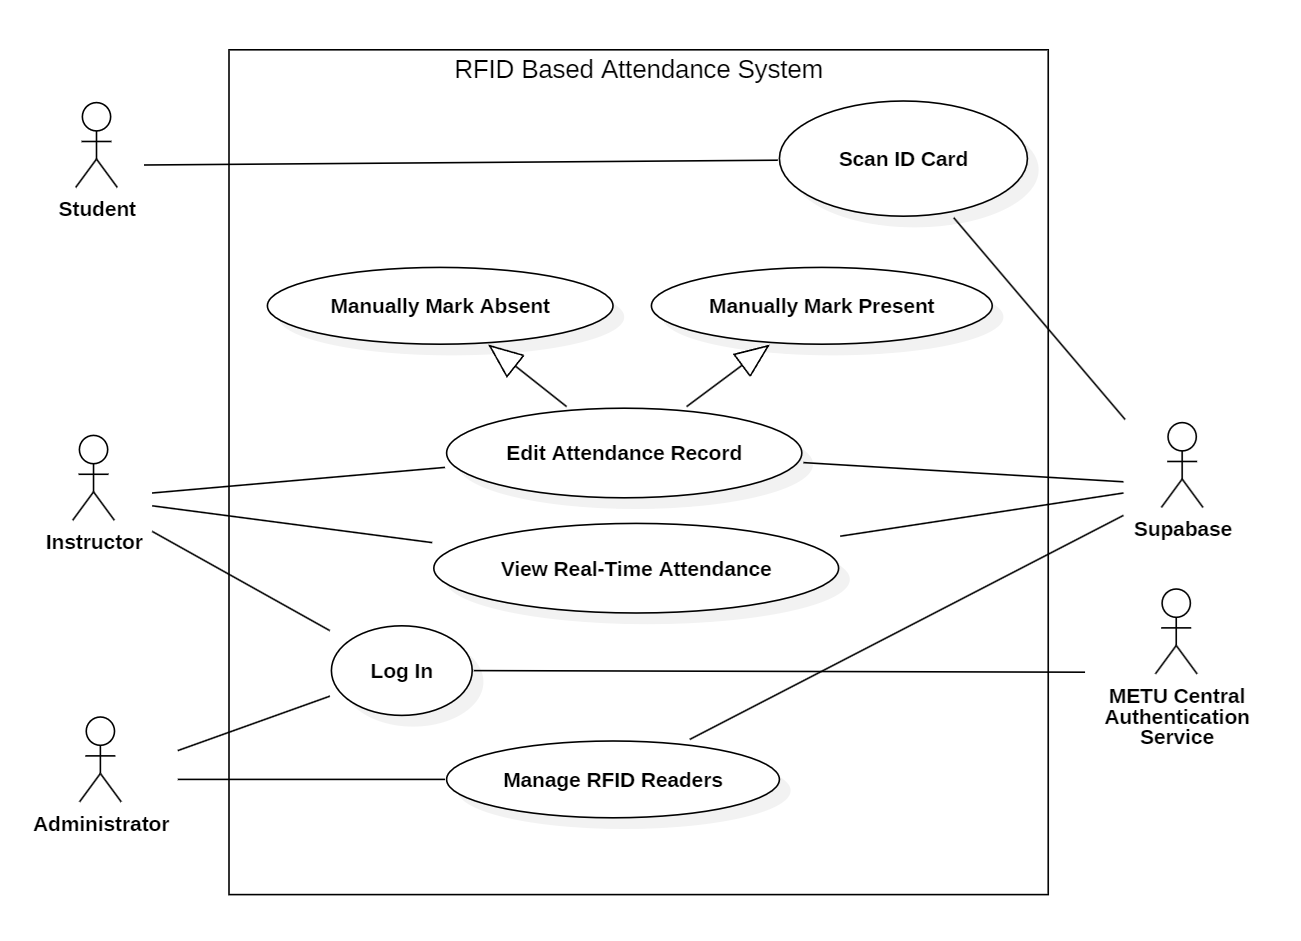
\includegraphics[width=\linewidth]{usecase.png}
    \caption{Use case diagram.}
    \label{fig:usecase}
\end{figure}


\newpage
\subsection{Data Flow Diagram}

\begin{figure}[H]
    \centering
    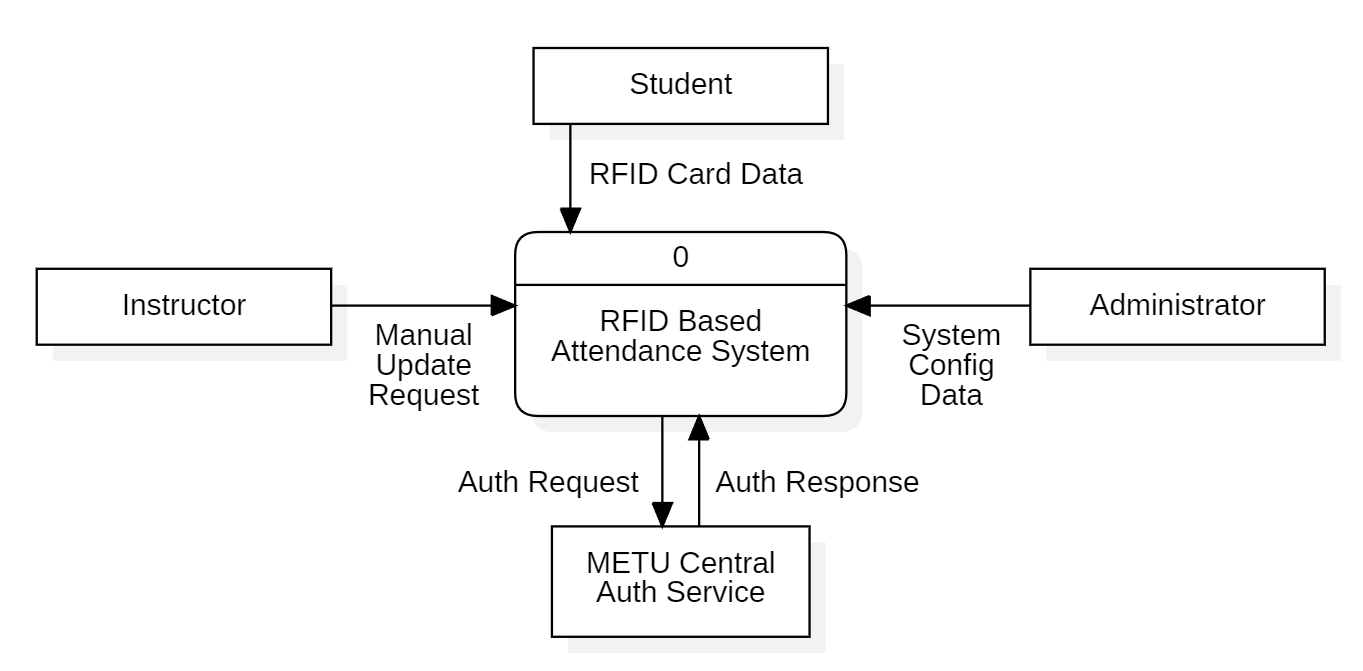
\includegraphics[width=0.75\linewidth]{dfd0.png}
    \caption{Level 0 data flow diagram.}
    \label{fig:dfd0}
\end{figure}

\begin{figure}[H]
    \centering
    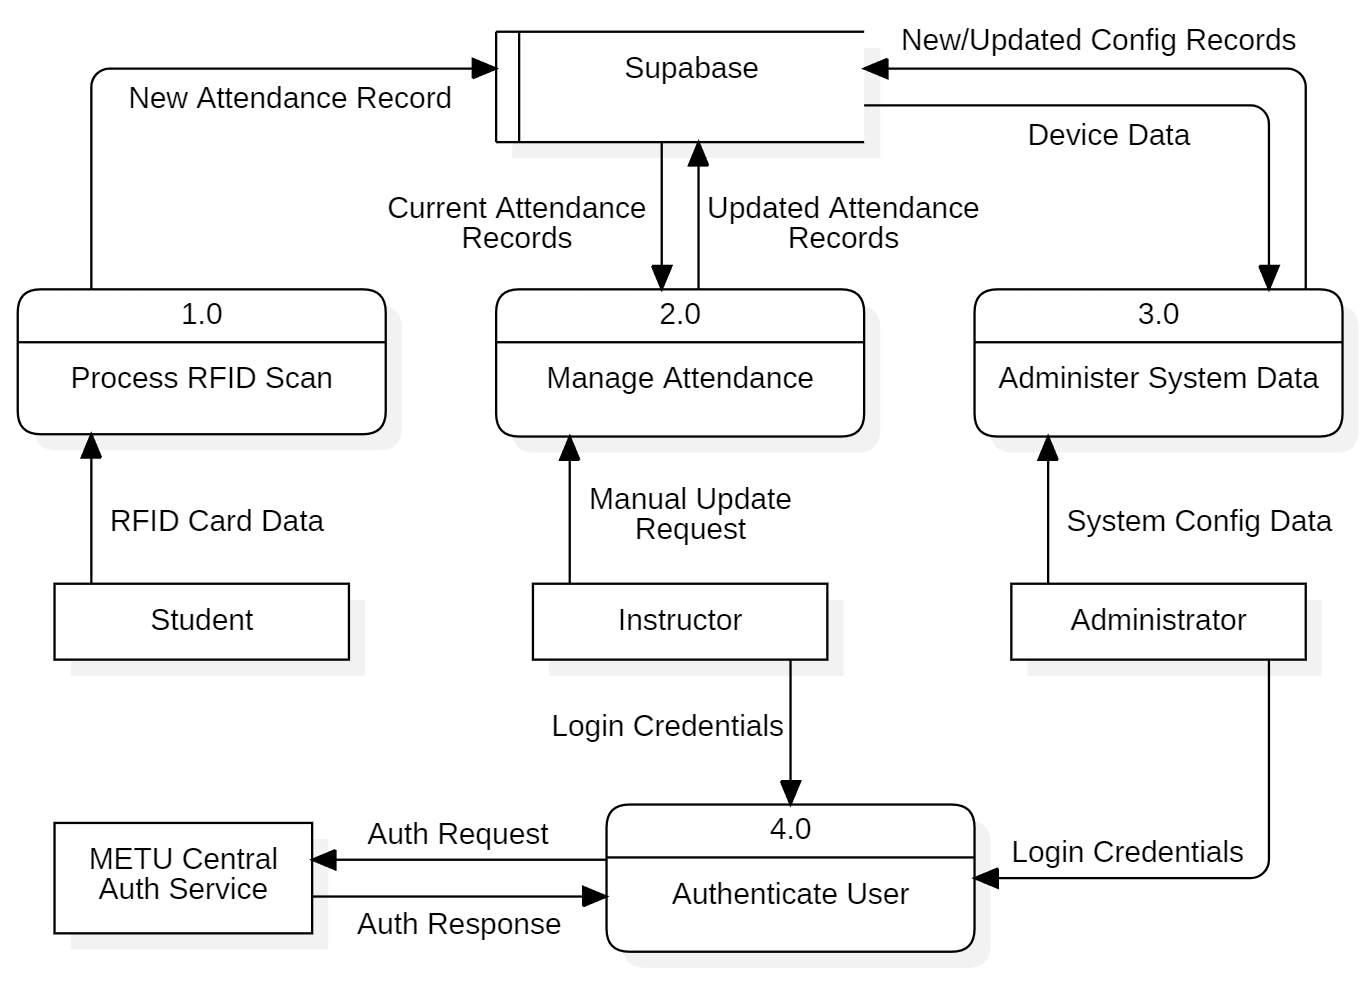
\includegraphics[width=0.75\linewidth]{dfd1.png}
    \caption{Level 1 data flow diagram.}
    \label{fig:dfd1}
\end{figure}



\newpage
\printbibliography[title={References}]

\end{document}
